\section{Avoid Latch}
\subsection{Introduction}%Purpose, brief intro, Contribution 
    \subsubsection{Latch}
    A latch is a component stores value until it's changed. But sometimes we may accidentally introduce unexpected latches in our design.
    \subsubsection{Drawback of Latch}
    \begin{enumerate}
        \item Latch may cause unnecessary resources to cost. Most FPGA chips don't have a latch component and will require many components to implement it, which is unnecessary.
        \item It might result in unstable output. When the input singal is unstable, the output of the latch will be unstable as well.
        \item The analysis of the circuit might be difficult because the latch make the circuit no longer pure combinational circuit.
    \end{enumerate}
    \subsubsection{Purpose of experiment}
    In this experiment, we will demonstrate how to introduce and avoid latches in three
    kinds of condition logic.
\subsection{Materials and Methods}%Show FPGA solution
    \subsubsection{To latch or not to latch}
        In the design, we introduce a latch by not giving the circuit a default output for not listed input. That is, if the input for any change don't meet the condition, the output will maintain it's previous input, and causing the latch.\par

        To avoid it, we simply add the default case back in the code.
    
    
\subsection{Results}%Show simulation and corresponding test results
    \subsubsection{Difference between Latch and no latch}
    \FloatBarrier
        \begin{figure}[]
                \FloatBarrier
            \centering
            \begin{subfigure}[h]{0.45\textwidth}
                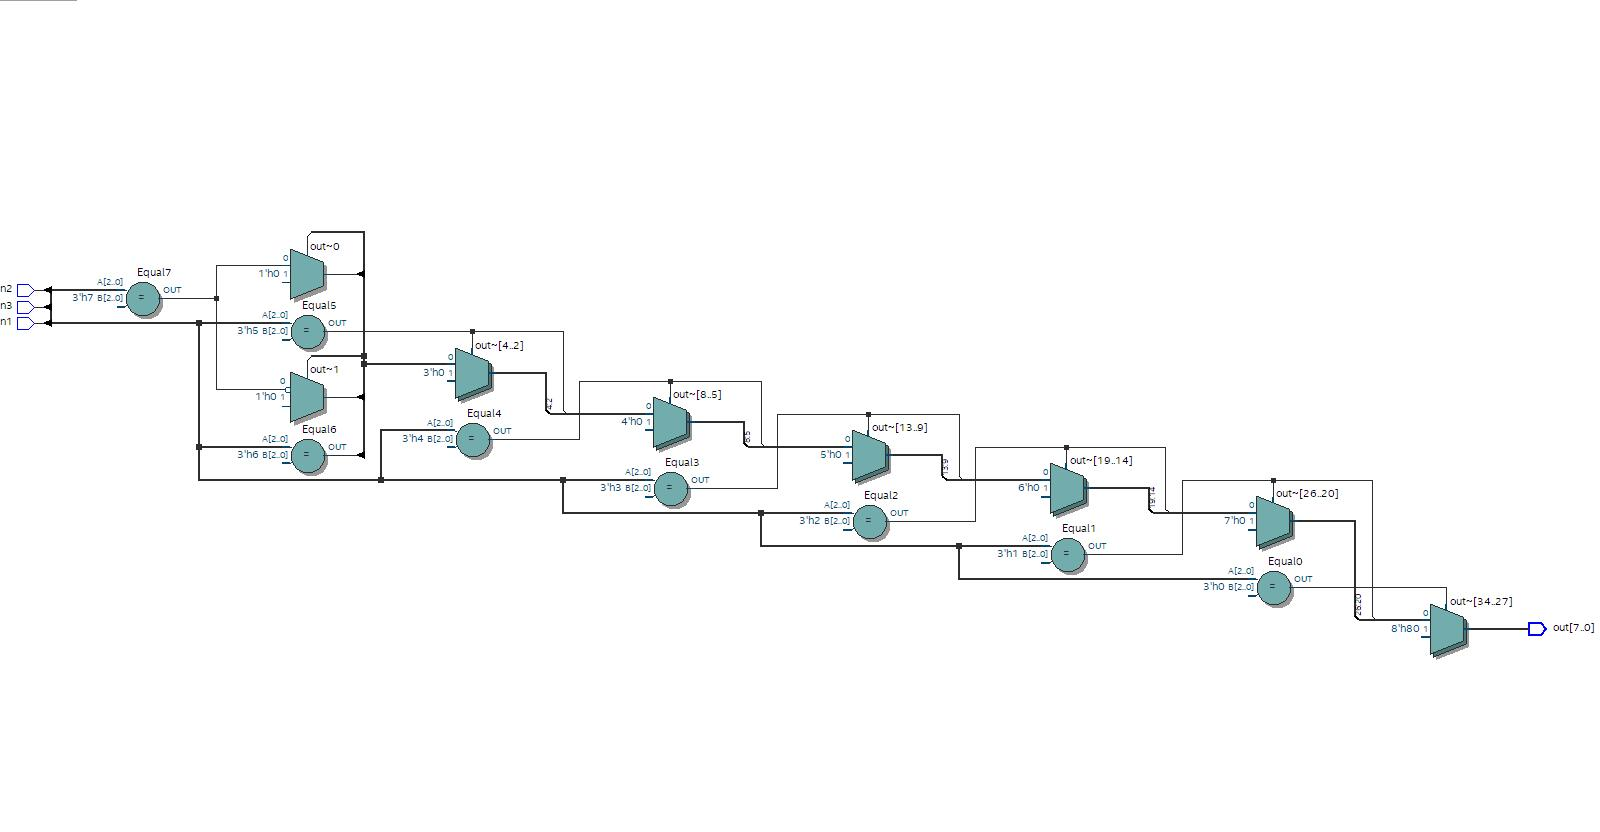
\includegraphics[width=1\linewidth]{22/Latch1.0.jpg}
                \caption{With out Latch}
            \end{subfigure}
            \begin{subfigure}[h]{0.45\textwidth}
                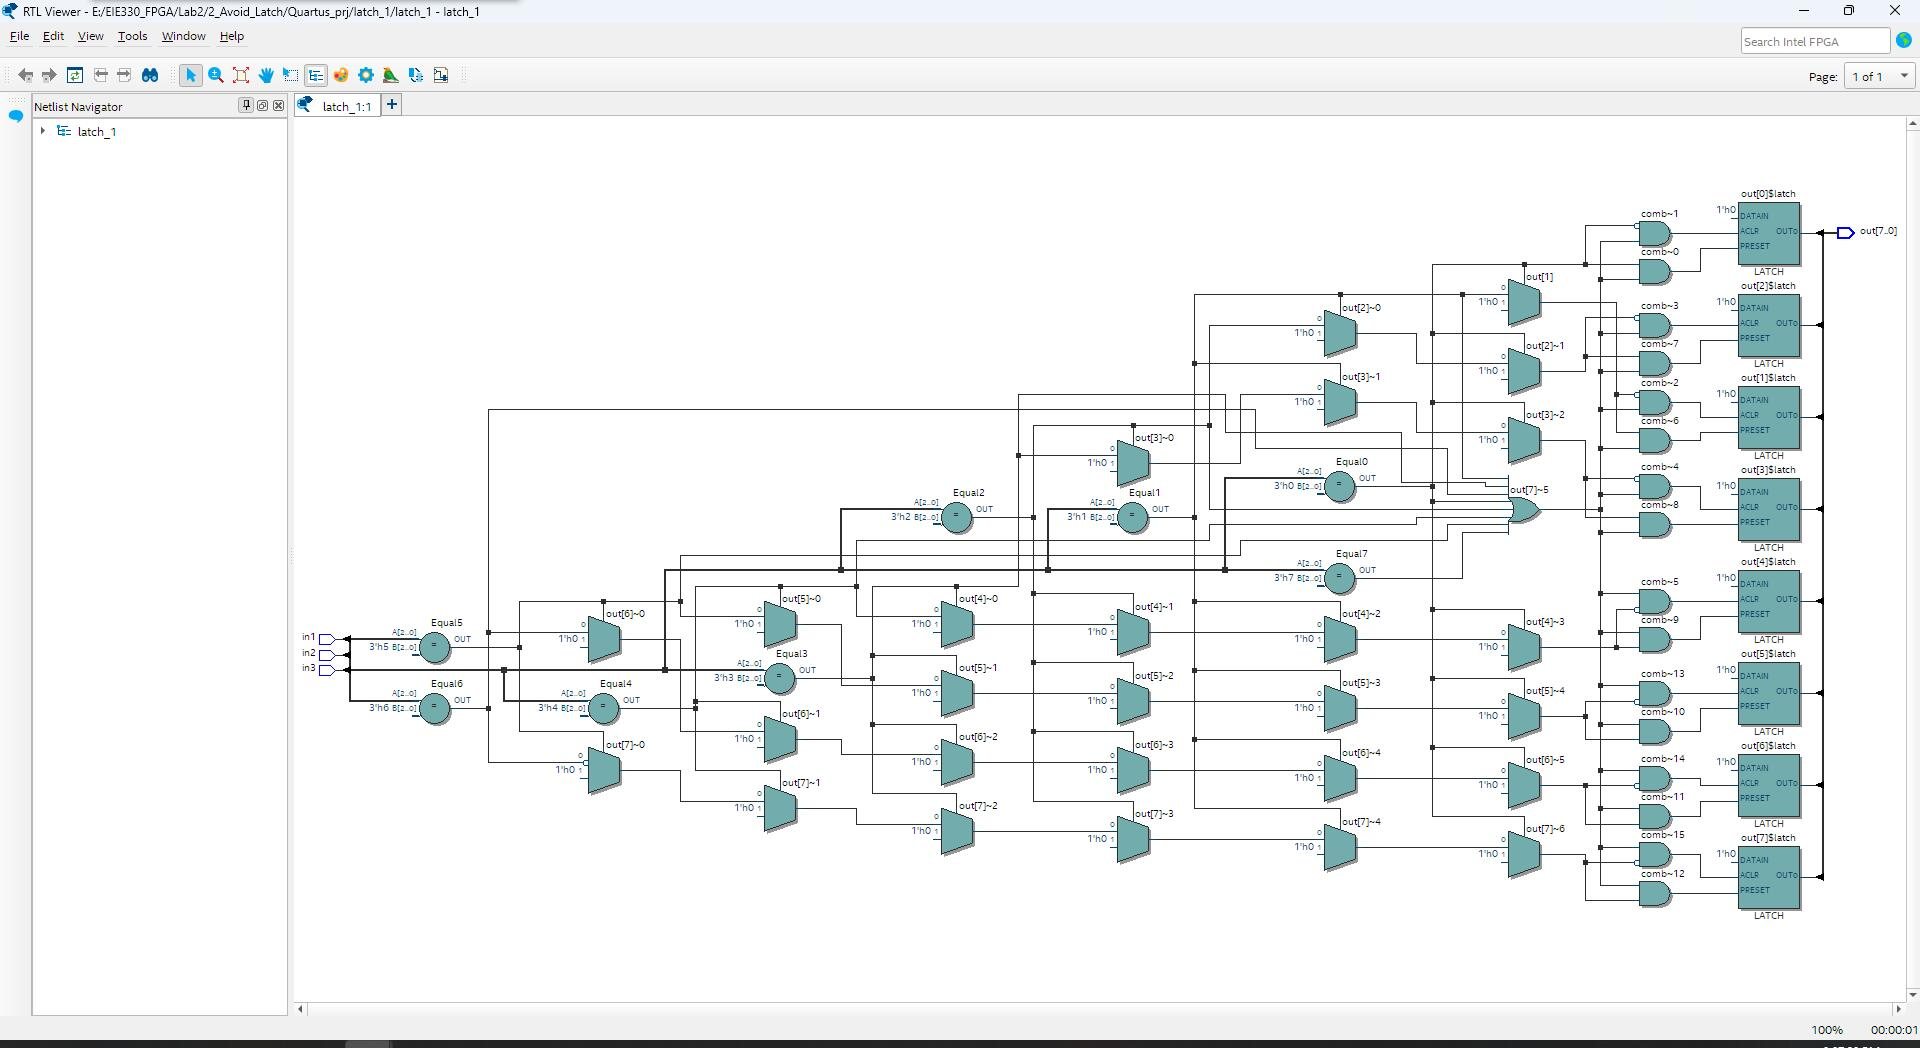
\includegraphics[width=1\linewidth]{22/Latch1.1.jpg}
                \caption{With out Latch}
            \end{subfigure}
            \caption{Latch 1}
            \label{fig:Latch1}
                    \FloatBarrier
        \end{figure}

        \FloatBarrier
        \begin{figure}[h!]
            \centering
            \begin{subfigure}[h]{0.45\textwidth}
                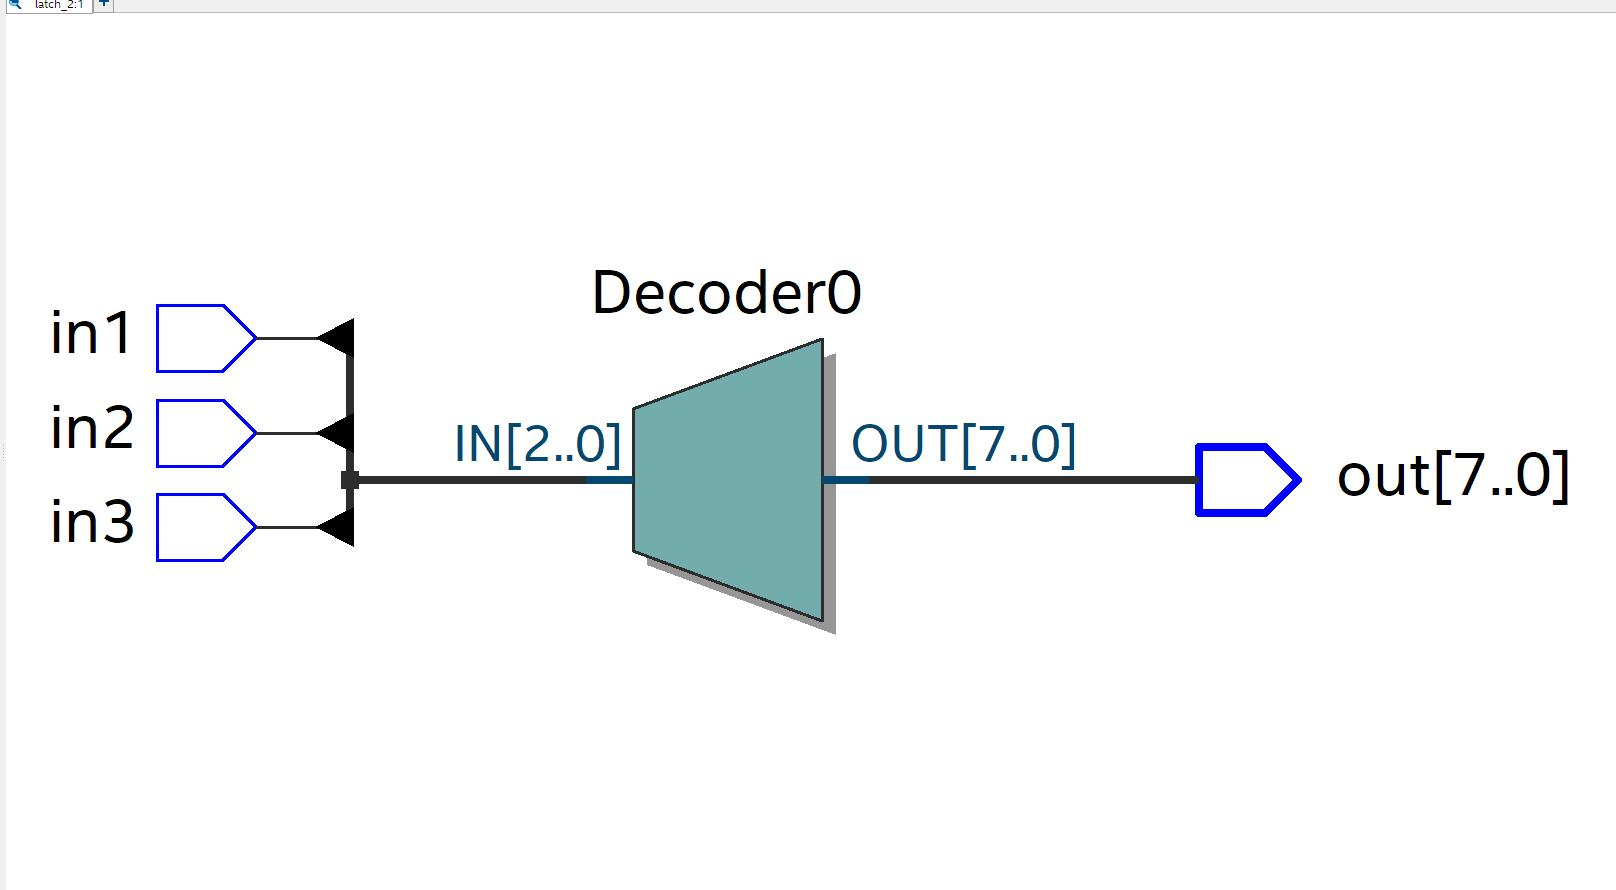
\includegraphics[width=1\linewidth]{22/latch2.0.jpg}
                \caption{With out Latch}
            \end{subfigure}
            \begin{subfigure}[h]{0.3\textwidth}
                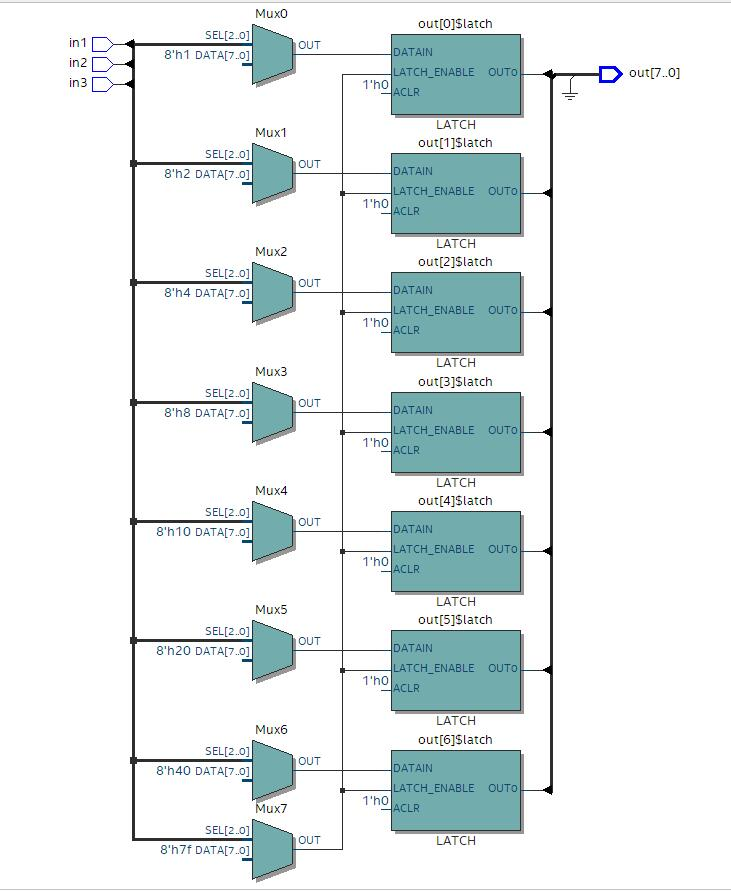
\includegraphics[width=1\linewidth]{22/latch2.1.jpg}
                \caption{With out Latch}
            \end{subfigure}
            \caption{Latch 2}
            \label{fig:Latch1}
        \end{figure}
                \FloatBarrier

                \FloatBarrier
        \begin{figure}[h!]
            \centering
            \begin{subfigure}[h]{0.45\textwidth}
                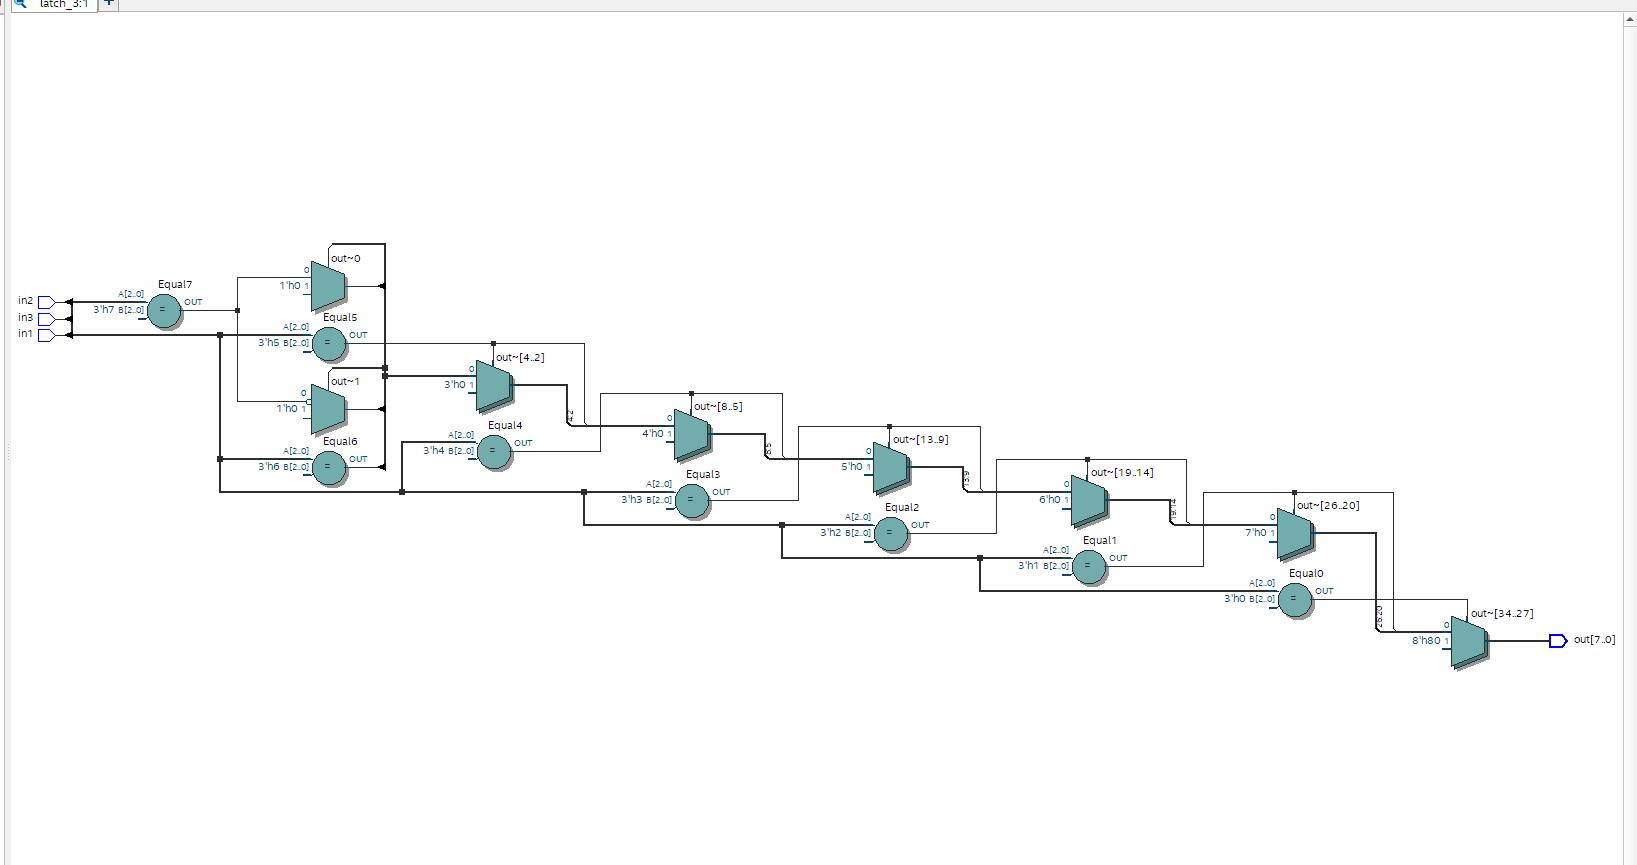
\includegraphics[width=1\linewidth]{22/latch3.0.jpg}
                \caption{With out Latch}
            \end{subfigure}
            \begin{subfigure}[h]{0.45\textwidth}
                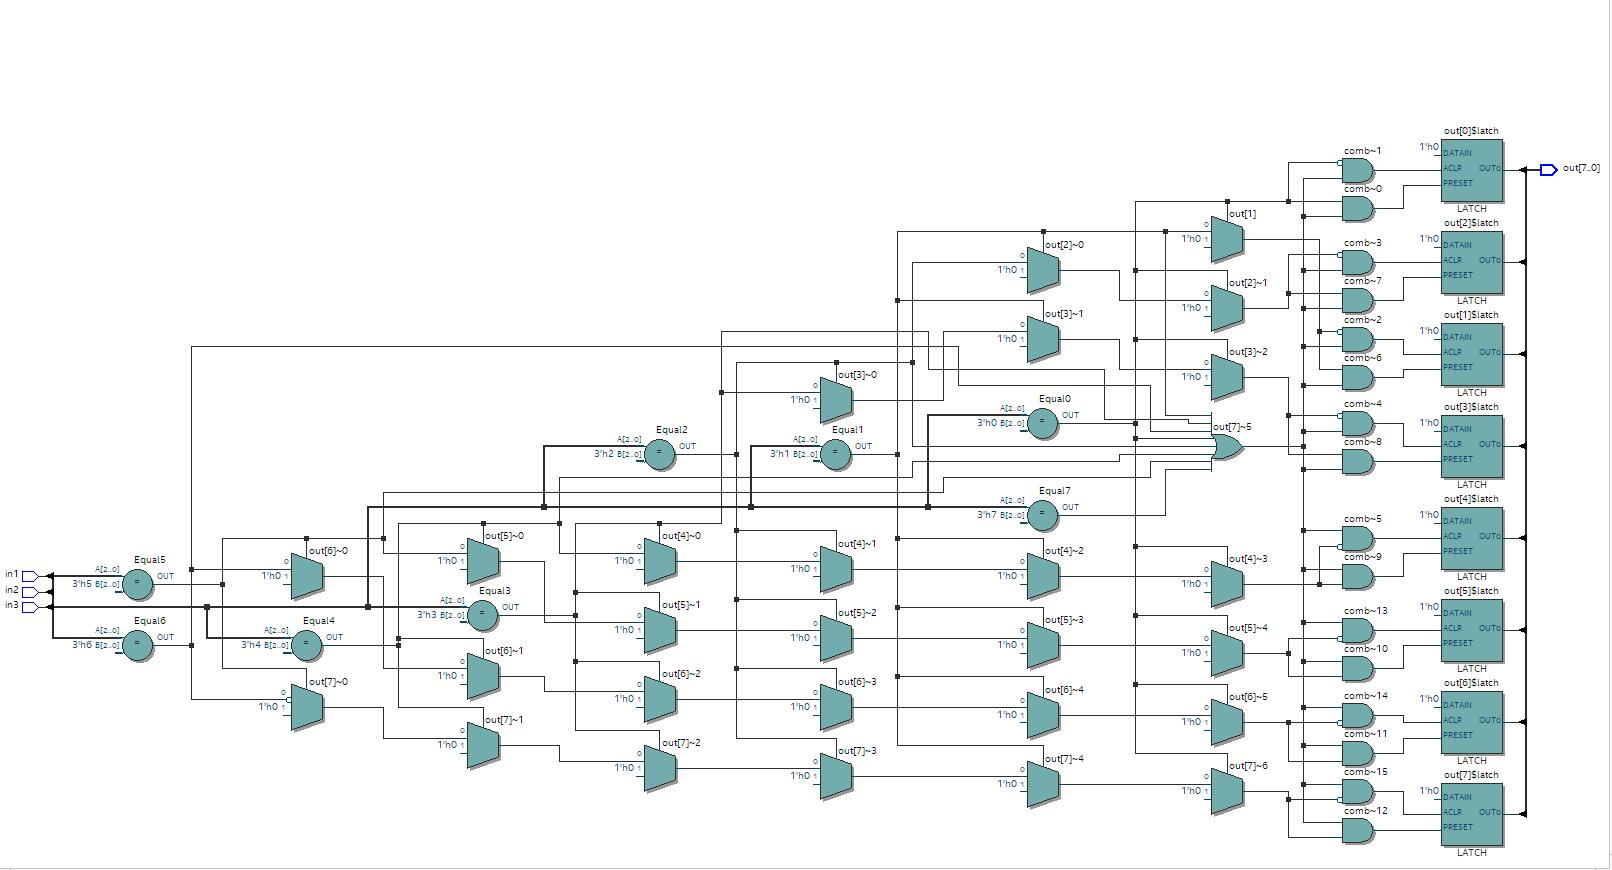
\includegraphics[width=1\linewidth]{22/latch3.1.jpg}
                \caption{With out Latch}
            \end{subfigure}
            \caption{Latch 3}
            \label{fig:Latch1}
        \end{figure}
                \FloatBarrier
    \subsubsection{Discussion}
        According to the figure, we can see the latch will overcomplicate the circuit that is meant
        to be very simple.\par

        \subsubsection{Drawback of Latch}
        Latch may cause unnecessary resources to cost. Most FPGA chips don't have a latch component and will require many components to implement it, which is unnecessary.
        Latch might result in unstable output. When the input singal is unstable, the output of the latch will be unstable as well.
        The analysis of the circuit might be difficult because the latch make the circuit no longer pure combinational circuit.
        \end{enumerate}
\subsection{Conclusion}
    
    
\subsection{Appendices}%References and Appendices
    The code in this experiment referenced the following sources (IEEE Style):\par
    \begin{thebibliography}{9}
        \bibitem{Avoid_Latch}% Identifier for intext citation
        pikipity, Aug, 2024, "FPGA-Laboratory/../2$\_$Avoid\_Latch,"~distributed on Github, 
            \url{https://github.com/pikipity/FPGA-Laboratory/tree/main/Lab2/2_Avoid_Latch/RTL}
        \bibitem{testbench_code}% Identifier for intext citation
         pikipity, Aug, 2024, "FPGA-Laboratory/../2$\_$Avoid\_Latch,"~distributed on Github, 
            \url{https://github.com/pikipity/FPGA-Laboratory/tree/main/Lab2/2_Avoid_Latch/Sim}
    \end{thebibliography}
    %\subsubsection{Appendices}%This optional section can include codes, raw data, calculations, additional graphs, and other supplementary material that is relevant but not essential to the main report.